\documentclass{ML}

% 姓名,学号
\infoauthor{朱明彦}{1160300314}

% 课程类型,实验名称
\infoexp{课程类型}{实验三}

\infoschool{计算机学院}{杨东华、王金宝}

\begin{document}
\maketitle

\tableofcontents
\newpage

\begin{center}
    \textbf{\zihao{3} 实验三 \  图数据分析}
\end{center}

\section{实验目的}
掌握大图数据计算平台的原理、架构和工作机制,理解大图计算平台的各项功能,包括数据载入、大图数据划分原理和大图计算。
能够编写大图数据计算平台中的常用图分析方法(PageRank, SSSP)程序。
\section{实验环境}
\begin{itemize}
\item Ubuntu 16.04.5
\item Java 1.8.0\_181
\end{itemize}
\section{实验过程及结果}
\subsection{项目架构}
\subsubsection{\texttt{Master}及其子类}
\begin{figure}[htb]
    \centering
    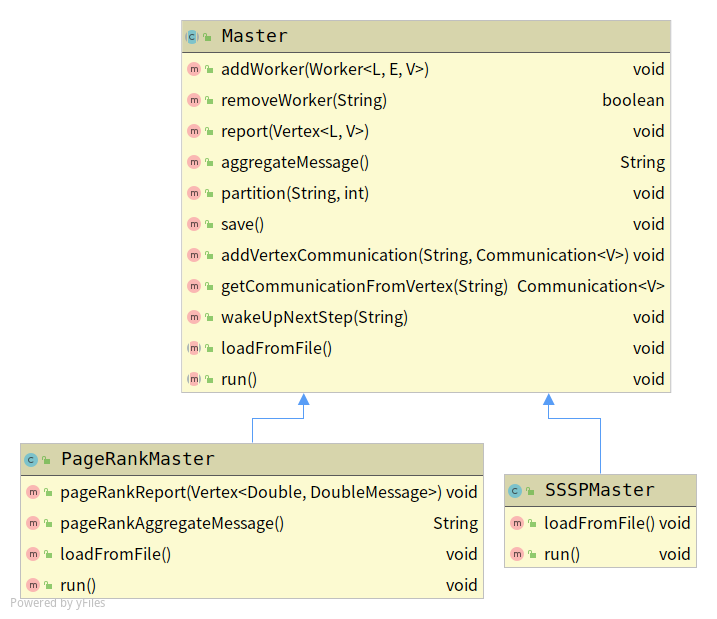
\includegraphics[width=0.6\linewidth]{media/master.png}
    \caption{\texttt{Master}及其子类UML图}\label{fig:master}
\end{figure}
对于\texttt{Master}与其子类,模拟的是BSP模型中Master节点。其中需要处理的问题主要有完成所有worker中每个顶点的计算、在所有的顶点之间进行通信两个功能。
在实现时以\texttt{Master}为抽象类,其中最为重要的抽象函数即\texttt{run()},对于不同的应用如SSSP和PageRanking,只需要重写\texttt{run()}函数来
完成其相应逻辑即可,\texttt{master}包中的继承关系如图\ref{fig:master}所示。

对于\texttt{Master}类,其定义时共有三个泛型参数,分别为\texttt{L,顶点类型;E,边类型;V,消息类型},对于SSSP问题,其只需将对应的泛型参数改为\texttt{Integer, Integer, IntMessage}即可。
对于\texttt{Master}类中设计的函数及其功能如下:
\begin{itemize}
    \item \texttt{addWorker, removeWorker}分别用于在\texttt{Master}类中增加删除\texttt{worker}。
    \item \texttt{report, aggregateMessage}主要用于全局的消息的aggregate,具体参见 节。% TODO
    \item \texttt{partition}用于将图进行划分,其中的两个参数分别为图源文件路径以及划分的数量。
    \item \texttt{save}用于将\texttt{partition}的结果存储到外存中,每个划分一个源文件,每一条输出类似$u,v_0,v_1\dots,v_n$,其中$u$为源点,$v_i$为$u$的所有出边的目的点,分隔符为\texttt{tab}。
    \item \texttt{addVertexCommunication, getCommunicationFromVertex}分别用于增删每个顶点对应的\texttt{communication},关于\texttt{communication}详见\ref{sec:communication}节。
    \item \texttt{wakeUpNextStep}是将发送消息的接收节点在下一轮唤醒(转为active状态)。
\end{itemize}

对于\texttt{SSSPMaster}和\texttt{PageRankMaster}而言,其\texttt{run}函数具有很大的相似性(\textbf{即进行BSP过程的模拟}),本质上都是一轮轮执行Worker,直到所有的Worker都结束,再将每个顶点的计算
结果输出至外存中进行保存;\textbf{不同在于对于PageRanking应用,只需要将所有的\texttt{Vertex}保持active状态,执行指定轮数即可,而对于SSSP应用则对每个Worker的状态进行判断,并在下一轮开始
之前将利用\texttt{wakeUpNextStep}唤醒的worker转入工作状态。}

\subsubsection{\texttt{Worker}及其子类}\label{sec:worker}
\begin{figure}[htb]
    \centering
    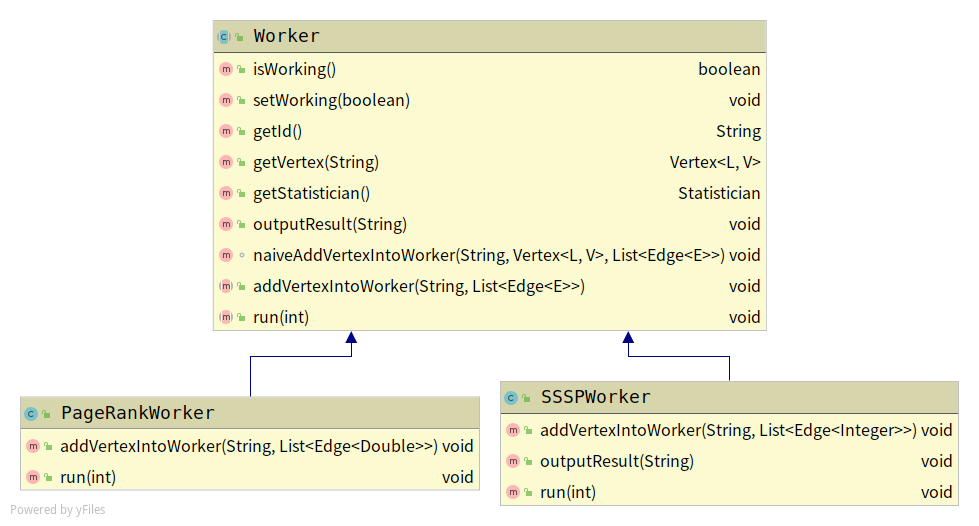
\includegraphics[width=0.7\linewidth]{media/worker.png}
    \caption{\texttt{Worker}及其子类UML图}\label{fig:worker}
\end{figure}
对于\texttt{Worker}及其子类,模拟的是BSP模型中的Worker节点,在其中需要维护每个Vertex的出边、消息队列(包括两个接收队列和一个发送队列,在本项目中利用\texttt{Communication}来实现,详见\ref{sec:communication}节)。
并且在接收到Master发送的消息后,串行在每个节点上执行\texttt{compute}函数,并将有更新的Vertex的产生的消息发送到对应的出边目的顶点即可。\texttt{worker}包中的继承关系如图\ref{fig:worker}所示。

对于\texttt{Worker}类,其定义时共有三个泛型参数,分别为\texttt{L,顶点类型;E,边类型;V,消息类型},对于SSSP问题,其只需将对应的泛型参数改为\texttt{Integer, Integer, IntMessage}即可,PageRanking问题同理。
在\texttt{Worker}类中设计函数及其功能如下所示:
\begin{itemize}
    \item \texttt{run(int)}用于在Worker上对其中的每个Vertex串行的执行\texttt{compute}函数。
    \item 一系列的\texttt{getter}和\texttt{setter}函数。
\end{itemize}

对于\texttt{SSSPWorker}而言,其\texttt{run}函数需要对其中每个当前接收队列不为空的Vertex执行\texttt{compute}函数,并将执行后为active的顶点,将更新后的信息发送至所有的出边的目的点;
而对于\texttt{PageRankWorker}而言,其\texttt{run}函数相对简单,只需要在第0轮super step利用对应的aggregator统计顶点的数目,在剩余轮数中对所有的顶点执行\texttt{compute}。

\subsubsection{\texttt{Vertex}及其子类}\label{sec:vertex}
\begin{figure}[htb]
    \centering
    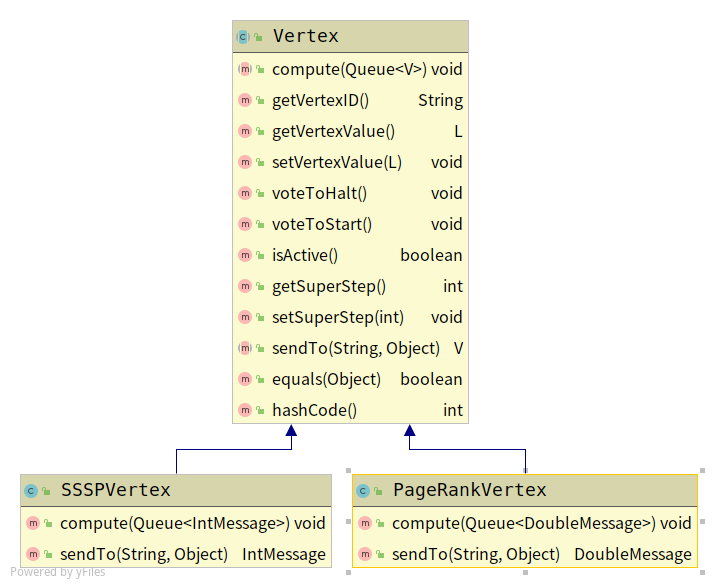
\includegraphics[width=0.7\linewidth]{media/vertex.png}
    \caption{\texttt{Vertex}及其子类UML图}\label{fig:vertex}
\end{figure}
对于\texttt{Vertex}及其子类,模拟的是BSP模型中的Vertex,其中基本类(抽象类)\texttt{Vertex}不参与运算,对于不同的应用分别重写\texttt{compute}函数即可。其中\texttt{Vertex}有
2个泛型参数,分别是\texttt{L,顶点类型;V,消息类型}。\texttt{vertex}包中的继承结构如图\ref{fig:vertex}所示。

\texttt{Vertex}中设计的函数及其功能如下:
\begin{itemize}
    \item \texttt{compute}即该顶点的需要执行的计算函数,对于不同的应用需要重写。
    \item \texttt{sendTo}用于产生该顶点需要发送的消息并将其返回,使用对应的worker进行发送。
    \item 一系列\texttt{getter}和\texttt{setter}函数等。
\end{itemize}

对于\texttt{SSSPVertex}的\texttt{compute}函数需要比较所有的接收消息中,是否存在比当前顶点的属性更小的信息,如果是则更新并将该顶点转为active状态,否则则将该顶点转为inactive状态。
对于\texttt{PageRankVertex}的\texttt{compute}计算,只需要在其中计算所有接收消息中值的和,然后在worker中计算$value = 0.15 / verticesNumber + 0.85 \times sum$\cite{pregel}。


\subsubsection{\texttt{Communication}}\label{sec:communication}
\begin{figure}[htb]
    \centering
    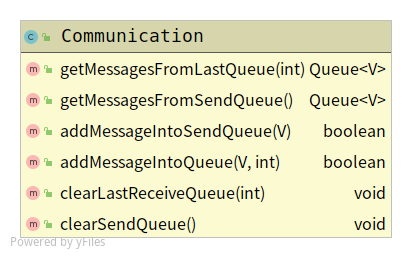
\includegraphics[width=0.5\linewidth]{media/Communication.png}
    \caption{\texttt{Communication}UML图}\label{fig:Communication}
\end{figure}

项目中实现Communication功能使用\texttt{Communication}类实现,其中有一个泛型参数\texttt{V,消息类型},有两个接收队列和一个发送队列,在使用时根据当前superStep的轮数
确定使用哪一个队列作为当前的接收队列(模2的结果进行选择)。\textbf{通过Master和Worker维护每个Vertex和其对应的\texttt{Communication}实例,来实现对于发送和接收消息过程的模拟。}


\subsubsection{\texttt{Combiner}类及其子类}
\begin{figure}[htb]
    \centering
    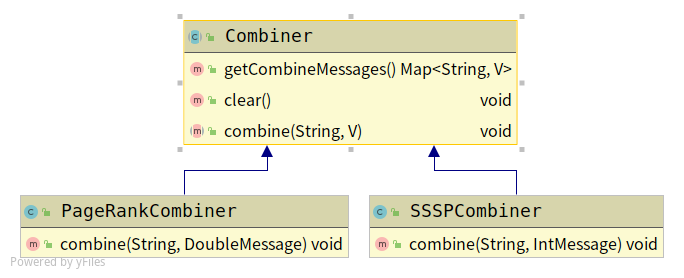
\includegraphics[width=0.7\linewidth]{media/combiner.png}
    \caption{\texttt{Combiner}及其子类UML图}\label{fig:combiner}
\end{figure}
\texttt{Combiner}及其子类用于将多条发送至同一Vertex的信息进行合并,对于不同的应用可以有不同的合并方式,在相应的子类中重写\texttt{combine}函数即可,
然后利用其中的维护的接收Vertex和信息的Map来实现减少通信数量的作用。\texttt{Combiner}与\texttt{Worker}结合使用,每个\texttt{Worker}中可以有
至多一个\texttt{Combiner},其继承关系如图\ref{fig:combiner}所示。

对于不同应用的\texttt{combine}函数的作用不同,分别有如下功能,
\begin{itemize}
    \item 对于\texttt{SSSPCombiner}而言,\texttt{combine}函数对于发往同一个目的顶点的信息,\textbf{取其中较小的信息}保留。
    \item 对于\texttt{PageRankCombiner}而言,\texttt{combine}函数对于发往同一目的地的信息\textbf{取和}保留。
\end{itemize}

\subsubsection{\texttt{Aggregator}及其子类}
\begin{figure}[htb]
    \centering
    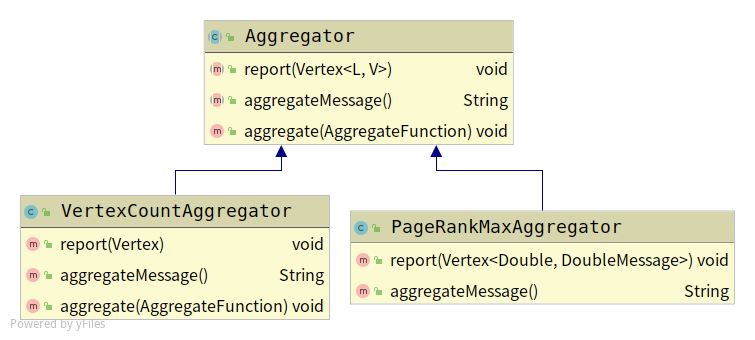
\includegraphics[width=0.7\linewidth]{media/aggregator.png}
    \caption{\texttt{Aggregator}及其子类UML图}\label{fig:aggregator}
\end{figure}
\texttt{Aggregator}及其子类用作统计全局信息,在本项目中主要使用其进行全局节点数目的统计和在执行完PageRanking后进行Rank的TopK统计。继承关系
如图\ref{fig:aggregator}所示,由于使用到全局信息,所以\texttt{Aggregator}与\texttt{Master}节点结合使用,并且对于每个\texttt{Master}
至多与1个\texttt{Aggregator}结合使用。

对于两种不同的应用,分别有不同的函数实现,
\begin{itemize}
    \item \texttt{VertexCountAggregator}用于统计全局的节点数目,故在\texttt{report}对其维护的Vertex数量进行自增即可。
    \item \texttt{PageRankMaxAggregator}用于全局的PageRank中TopK的统计,所以在其中维护了一个大小为K的小顶堆,在不足K个时将每个顶点均加入
    堆中,达到K个时则判断当前堆顶元素的Rank是否比新来的Vertex的Rank高,如果新来的更高则弹出堆顶元素,加入新来元素,否则直接舍弃堆顶元素即可。
\end{itemize}

\subsection{图分析算法实现}
SSSP的实现和PageRank的实现区别主要在\texttt{Worker}和\texttt{Vertex}实现的区别,接下来分别进行说明。
\subsubsection{SSSP的实现}
\texttt{SSSPVertex}在接收到消息时将自身转为active状态,但通过消息队列计算当前的最短距离没有发生改变,就再将自身转为inactive状态。
关于\texttt{SSSPWorker}的区别,在\ref{sec:worker}节有详细说明。
\subsubsection{PageRank的实现}
\texttt{PageRankWorker}只需在指定轮数之内保持active状态,将更新后的信息发送给所有的出边目的顶点即可,到达制定轮数之后转为inactive即可。
关于\texttt{PageRankWorker}的具体实现,见\ref{sec:worker}节说明。
\section{实验心得}
总的来说,模拟Pregel\cite{pregel}的难度不大,而在于理清各个类之间的关系,以及模拟BSP模型时注意模拟各个方法的调用顺序。建议在之后的实验里可以
适当增大该实验的难度,比如多线程并行模拟BSP模型,线程数为worker数量。
\appendix

% \section{源代码}
% \section{参考文献}
\begin{thebibliography}{20}
    \bibitem{pregel} Malewicz, G., Austern, M. H., Bik, A. J., Dehnert, J. C., Horn, I., Leiser, N., \& Czajkowski, G. (2010, June). Pregel: a system for large-scale graph processing. In Proceedings of the 2010 ACM SIGMOD International Conference on Management of data (pp. 135-146). ACM.
    % \bibitem{employee_name} 中国最常见名字前50名, \texttt{https://www.sohu.com/a/164406113\_367620}
    % \bibitem{employee_id} 身份证号在线生成器, \texttt{https://www.tinysoft.org/}
\end{thebibliography}

\end{document}
